
%(BEGIN_QUESTION)
% Copyright 2006, Tony R. Kuphaldt, released under the Creative Commons Attribution License (v 1.0)
% This means you may do almost anything with this work of mine, so long as you give me proper credit

Shown here is the mechanism for a simplified (no amplifying relay, no bias spring) proportional-only pneumatic controller:

$$\includegraphics[width=15.5cm]{i01596x01.eps}$$

What needs to be changed or adjusted in this mechanism to {\it decrease} the controller's proportional band?  Also, determine whether this controller is {\it direct-acting} or {\it reverse-acting}.

\vskip 20pt \vbox{\hrule \hbox{\strut \vrule{} {\bf Suggestions for Socratic discussion} \vrule} \hrule}

\begin{itemize}
\item{} Is this a {\it force-balance} mechanism or a {\it motion-balance} mechanism?  How can you tell for certain?
\item{} Could the mechanism be modified to convert it into the other type of balance?  If so, how?
\end{itemize}

\underbar{file i01596}
%(END_QUESTION)





%(BEGIN_ANSWER)

To decrease the controller's proportional band (increase its gain), move the fulcrum further to the left:

$$\includegraphics[width=15.5cm]{i01596x02.eps}$$

This controller mechanism is direct-acting.

%(END_ANSWER)





%(BEGIN_NOTES)

Moving the fulcrum to the left makes the output bellows have to react more aggressively to changes in error (PV $-$ SP), because its force works on a shorter moment arm length.  This constitutes an increased gain, which is the same as saying a decreased proportional band.

Some students might think the opposite, because they see moving the fulcrum to the left as decreasing baffle motion relative to the nozzle, therefore decreasing output response.  While this is correct with regard to motion, it is not correct with regard to {\it force}.  Since this mechanism is force-balance and not motion-balance, we must think in terms of forces.

One thought experiment useful in shattering this misconception is to envision the feedback bellows not existing.  If there was no feedback bellows, would the fulcrum position really matter at all?  Of course not, since {\it any} error would force the baffle far enough to achieve output saturation.  It is the force feedback that makes this controller mechanism work, not apparent motion.

Remind your students that an amplified baffle/nozzle assembly need only move a couple thousandths of an inch to achieve full output saturation!

%INDEX% Control, proportional: pneumatic force-balance controller

%(END_NOTES)


